\documentclass[12pt]{article}
\usepackage[T1]{fontenc}
\usepackage[utf8]{inputenc}
\usepackage{graphicx}
\usepackage[spanish]{babel}
\usepackage{hyperref}
\usepackage{blindtext}
\usepackage{setspace}
\setstretch{1.5}
\usepackage{listings}
\usepackage{xcolor}

\definecolor{codegreen}{rgb}{0,0.6,0}
\definecolor{codegray}{rgb}{0.5,0.5,0.5}
\definecolor{codepurple}{rgb}{0.58,0,0.82}
\definecolor{backcolour}{rgb}{0.95,0.95,0.92}

\lstdefinestyle{mystyle}{  
    commentstyle=\color{codegreen},
    keywordstyle=\color{magenta},
    numberstyle=\tiny\color{codegray},
    stringstyle=\color{codepurple},
    basicstyle=\ttfamily,
    breakatwhitespace=false,         
    breaklines=false,                 
    captionpos=b,                    
    keepspaces=true,                  
    showspaces=false,                
    showstringspaces=false,
    showtabs=false,                  
    tabsize=1
}


\lstset{language=bash}
\lstset{style=mystyle}


\begin{document}

	\begin{titlepage}
		\centering
		{\bfseries\LARGE Instituto Politécnico Nacional \par}
		\vspace{0cm}
		{\Large Escuela Superior de Cómputo  \par}
		\vspace{1cm}
		{\scshape\Huge Documentación Práctica 1 \par}
		\vspace{1cm}
		{\Large Autor: \par}
		{\Large Contreras Barrita José Roberto \par}
		\vspace{1cm}
		{\Large Materia: \par}
		{\Large Ingeniería de Software \par}
		\vspace{1cm}
		{\Large Grupo: \par}
		{\Large 3CV17 \par}
		\vspace{1cm}
		{\Large Profesor: \par}
		{\Large Vélez Saldaña Ulises \par}
	\end{titlepage}
	
	\tableofcontents
	\clearpage
	
	\section{Diseño}
		Para la creación de esta práctica se tuvieron que realizar suposiciones y decisiones para poder realizar el desarrollo. A continuación se describirán.
		
		\subsection{Tecnologías}
			Se decidió crear una aplicación que se ejecute en consola en un entorno Linux por lo cual se empleo el lenguaje de programación \textbf{Python} para la creación del código debido a que es un lenguaje de aprendizaje sencillo, de código abierto y que su interprete se encuentra instalado en todas las distribuciones Linux por lo que su ejecución no implicará ningún problema.
			
			
			Una funcionalidad del programa es poder almacenar los datos de los clientes por lo cual se optó por utilizar bases de datos para la conservación y fácil manejo de la información, en este caso se utilizó el gestor de bases de datos \textbf{SQLite} el cual tiene su implementación en Python y no necesita la instalación de algún otro software extra como en el caso de otros gestores de bases de datos.
			
		\subsection{Diseño y estructura del proyecto}
			El manejo del programa se hará mediante un menú de opciones en el que el usuario dará como entrada mediante la consola el número de la opción a desear, este menú aparecerá después de realizar cada operación y se quitará una vez el usuario seleccione la opción de salir, para este programa solo es necesario el uso del teclado. En cuestión de seguridad los usuarios solo podrán ingresar al sistema si conocen la clave de acceso. Para el manejo de la información se creo una base de datos con dos tablas, la tabla clients donde se almacena la información de los clientes que registre el usuario y la tabla sec donde se almacena la contraseña de acceso al programa.
			El proyecto contará con una estructura definida por los siguientes elementos:
			\begin{itemize}
				 \item\textbf{ docs:} Directorio que contendrá la documentación del proyecto en un archivo PDF.
				\item \textbf{ res:} Directorio en el que se guardarán todos los recursos necesarios para que le programa funcione correctamente. Aquí estará el archivo necesario para el funcionamiento de la base de datos, este archivo es portable por si se desea usar el programa en otro ordenador con la información ya creada. 
				\item \textbf{ src:} Directorio donde se encuentra el código fuente del programa y tiene los archivos a interpretar, aquí se decidió codificar en base a módulos dónde se crearon los siguientes dos archivos:
				\begin{itemize}
	  			\item Archivo \textbf{main.py}: Contiene la lógica principal y las instrucciones para interactuar con el usuario. Hace uso del modulo dbmanager.
	  			\item Archivo \textbf{dbmanager.py}: Modulo que contiene todas las operaciones para el manejo de la base de datos.
	  			
				\end{itemize}	
				
				\item \textbf{README.txt:} Archivo que da una breve descripción del programa, su estructura y su instalación.
				\item \textbf{run.sh:} Script en bash que se encarga de correr el programa.
			\end{itemize}
		\newpage
		\subsection{Estructura de los datos}
			Se tomaron ciertas decisiones al momento de definir los tipos de datos. Para el alias se considera un texto de máximo 10 dígitos considerando espacios. El nombre deberá tener máximo una longitud de 30 caracteres y los apellidos una longitud máxima de 20 caracteres cada uno. La razón social no tiene un limite de caracteres y acepta la mayoría de los caracteres.
			\\
			El RFC tiene una longitud máxima de 13 caracteres ya que es la longitud máxima que puede tener un RFC en México. El número telefónico deberá tener una longitud de 10 dígitos debido a que es el nuevo estándar en México y el correo tendrá una longitud máxima de 50 caracteres considerando el dominio.
			En el apartado de seguridad la clave de accesos deberá tener máximo 50 caracteres y no debe tener espacios de preferencia.
					
			
	\newpage	
	\section{Descarga y ejecución}
		Para este apartado se necesitara noción de comandos en Linux.
		\subsection{Requisitos del sistema}		
		Para la instalación y ejecución de este programa deberá tener instalado el software de control de versiones \textbf{git} y el interprete de Python en este caso en su versión \textbf{python3}. 
		
		\subsection{Descarga}		
		Abriremos la terminal y nos dirigiremos a la ruta donde queremos guardar los archivos del programa. Una vez ubicados ahí ejecutaremos el siguiente comando para descargar todo lo necesario.
		
		\begin{lstlisting}
		git clone https://github.com/jcontrerasroberto/isw-practica1.git
		\end{lstlisting}
		
		\subsection{Ejecución}	
		Después de descargar el repositorio ingresaremos a la carpeta que contiene los archivos del programa
		\begin{lstlisting}
		cd isw-practica1 
		\end{lstlisting}
		\newpage
		 Otorgamos permisos de ejecución al script run.sh y lo corremos
		
		\begin{lstlisting}
		chmod +x run.sh
		./run.sh
		\end{lstlisting}
		O en su defecto corremos el programa directamente con el comando:
		\begin{lstlisting}
		python3 src/main.py
		\end{lstlisting}
		
		De ahora en adelante solo tendrás que entrar a la carpeta isw-practica1 y correr el script run.sh para iniciar el programa
		
	\newpage	
	
	\section{Funcionamiento y pruebas}
	
		La primera vez que ejecutemos el programa pedirá que ingresemos una nueva contraseña de seguridad. Ingresamos la contraseña y damos enter.
	
		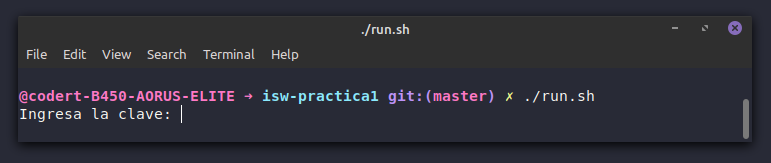
\includegraphics[scale=0.7]{cap1}\newline

		Las siguientes veces que iniciemos el programa pedirá la contraseña creada la primera vez.
	
		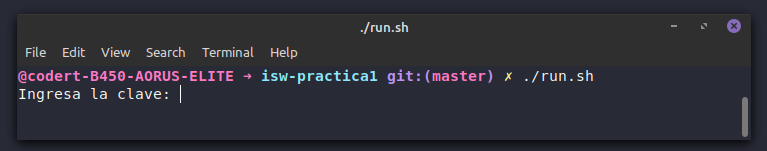
\includegraphics[scale=0.7]{cap2}\newline

		Después de ingresar la contraseña observaremos un menú donde el usuario puede escoger.
	
		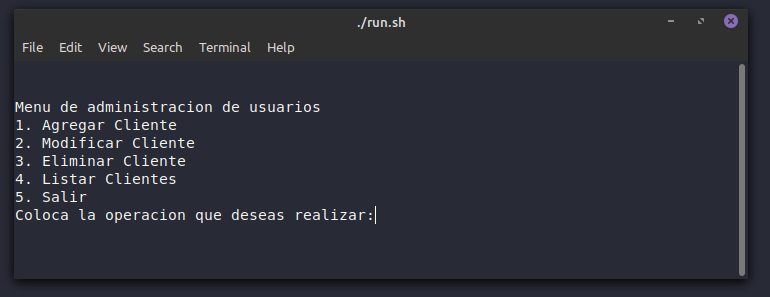
\includegraphics[scale=0.7]{cap3}
	
		\subsection{Agregar cliente}
			Para usar esta función ingresaremos \textbf{1} en el menú. El programa nos pedirá los datos, iremos ingresandolos y apretando enter hasta que se registre al usuario. 
			
			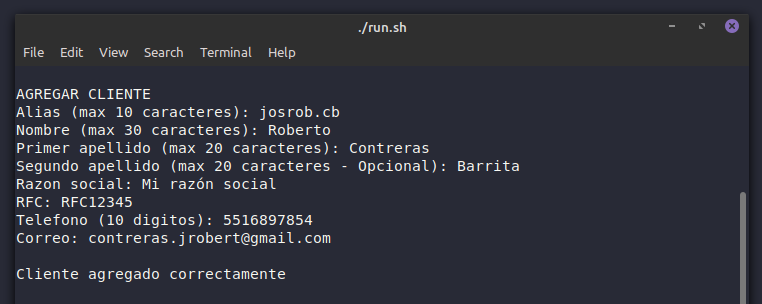
\includegraphics[scale=0.7]{cap4}
			
		\subsection{Modificar cliente}
			Para usar esta función ingresaremos \textbf{2} en el menú. El programa nos pedirá el alias al cliente a modificar y una vez que lo encuentre empezará a pedir los datos actualizados. Nota: Si no se quiere actualizar un campo solo dar enter dejando la entrada vaciá. 
			
			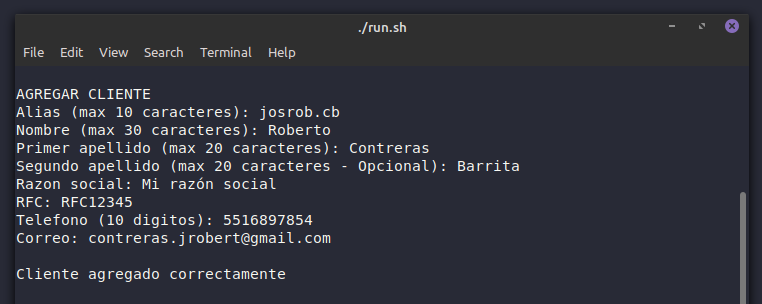
\includegraphics[scale=0.7]{cap4}\newline
	
	\newpage
	\section{Consideraciones}

\end{document}
